\documentclass[a4paper]{article}

%% Language and font encodings
\usepackage[english]{babel}
\usepackage[utf8]{inputenc}
\usepackage[T1]{fontenc}

%% Sets page size and margins
\usepackage[a4paper,top=3cm,bottom=2cm,left=3cm,right=3cm,marginparwidth=1.75cm]{geometry}

%% Useful packages
\usepackage{amsmath}
\usepackage{graphicx}
\usepackage[colorinlistoftodos]{todonotes}
\usepackage[colorlinks=true, allcolors=blue]{hyperref}

\title{Reporte Actividad 2}
\author{Jonás Valenzuela Terán}

\begin{document}
\maketitle

\begin{abstract}
El objetivo de la actividad es tener un primer acercamiento al lenguaje de programación Python así como el entorno Jupyter Notebook, que permiten una dinámica muy diferente de trabajo.
\end{abstract}

\section*{Descripción}

Jupyter Notebook es una aplicación web open-source, para crear y editar documentos con código "En vivo", esto es que se pueda correr el código de lenguajes como Python o R, mientras se crea, además facilita compartir archivos y puede usarse offline.

Se pueden añadir paquetes como Matplotlib para habilitar la graficación "en vivo", o la librería Pandas, que funciona para el análisis de datos, siendo capaz de ordenar datos, señalar lo importante, y adaptarlos para análisis, es importante para datos estadísticos de alto nivel, maneja la estructura básica de datos llamada DataFrame.

\section*{Ventajas y desventajas}
Jupyter Notebook en conjunto con Python y las librerias mencionadas, son muy útiles para realizar trabajos rápidos, análisis de datos, y compartir resultados, además es un ambiente amigable para usuarios sin conocimiento previo. Las desventajas son que esto añade complejidad, lo que hace difícil arreglar errores, o realizar proyectos grandes en colaboración.

\section*{Lo aprendido}
Aprendimos a cargar las librerias principales, leer archivos de datos, describir los datos, graficar de maneras diferentes, y como funciona la dinámica del lenguaje interpretado, que puede correr al ser indicado y reiniciar el kernel.

Se utilizaron datos meteorológicos de Yecora para realizar el análisis de sus datos:

\begin{center}

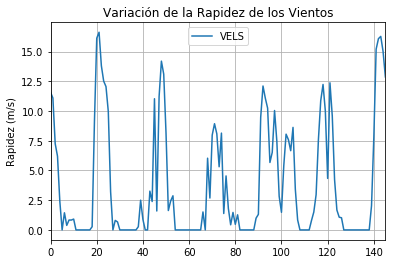
\includegraphics[height=4.5cm]{grafica1.png}

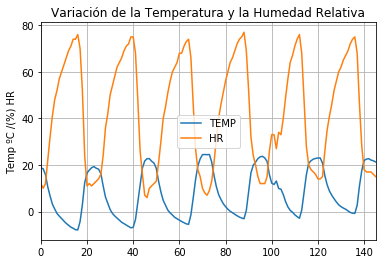
\includegraphics[height=4.5cm]{grafica2.png}

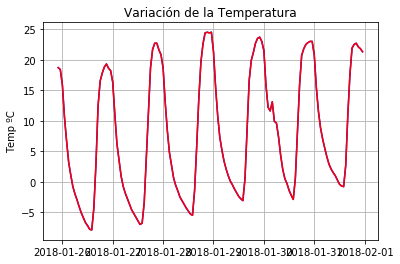
\includegraphics[height=4.5cm]{grafica3.png}

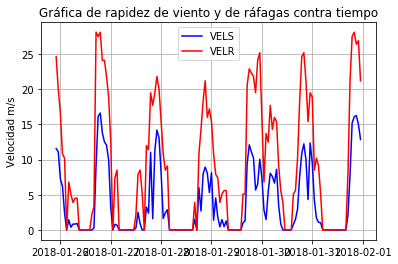
\includegraphics[height=4.5cm]{grafica4.png}

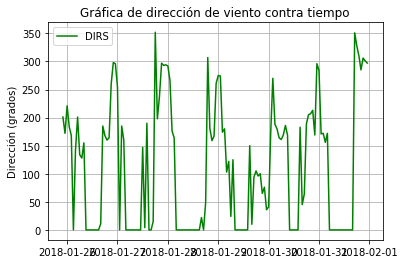
\includegraphics[height=4.5cm]{grafica5.png}

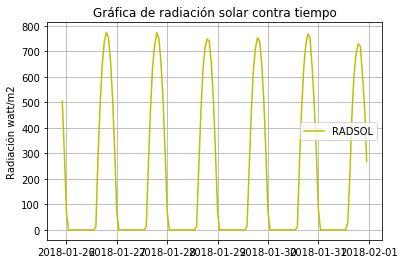
\includegraphics[height=5cm]{grafica6.png}

\end{center}


\section*{Apéndice}


\begin{itemize}
\item     ¿Cuál es tu primera impresión de Jupyter Notebook?

Es muy diferente a Fortran, es muy inmediato y gráfico.

\item     ¿Se te dificultó leer código en Python?

No, los comandos se explican por si mismos, son intuitivos.

\item     ¿En base a tu experiencia de programación en Fortran, que te parece el entorno de trabajar en Python?

Se me hace bien, es mejor para análisis rápidos, y es más fácil encontrar errores.

\item     A diferencia de Fortran, ahora se producen las gráficas utilizando la biblioteca Matplotlib. ¿Cómo fue tu experiencia?. 

Es muy cómodo tener integrado herramientas de graficación junto con el código, y no tener que recurrir a un programa externo y compilar cada cambio.

\item     En general, ¿qué te pereció el entorno de trabajo en Python? 

Me parece una buena herramienta para agregar a nuestras habilidades, ya que se adapta mejor a algunas tareas.

\item     ¿Qué opinas de la actividad? ¿Estuvo compleja? ¿Mucho material nuevo? ¿Que le faltó o que le sobró? ¿Qué modificarías para mejorar? 

Si es material y ambientes muy nuevos, pero afortunadamente son amigables con el usuario, y funcionan como uno lo espera.

\item     ¿Comentarios adicionales que desees compartir? 

Me agrada usar herramientas open-source que se usan muy frecuentemente en el ámbito profesional

\end{itemize}




\bibliographystyle{alpha}
\begin{itemize}
\item \textit{Introducción a pandas}. 7 de febrero 2018, de Programacion.net Sitio web: \textit{programacion.net}

\item Yassine Alouini. ( 2017). \textit{What are the pros and cons of using Python Jupyter versus a normal Python development environment?}. 7 de febrero 2018, de Quora Sitio web:\textit{ https://www.quora.com/What-are-the-pros-and-cons-of-using-Python-Jupyter-versus-a-normal-Python-development-environment}
\end{itemize}


\end{document}